\phantomsection
\section{写像}

\phantomsection
\subsection{写像の定義と例}

\phantomsection
\subsubsection{写像の定義}

いままでの数学の学習の過程で「関数\index{かんすう@関数}」という言葉に出会ったことがある読者もいるかもしれない.
そのような経験がある読者は「関数」と言われると,どのようなものが思い浮かぶであろうか.

関数の一般的な表現として「写像」がある\footnote{写像の始集合・終集合が$\mathbb{R}$など「数」の集合であるときに「関数」と呼ぶことが多い.}.厳密な写像の定義はのちに述べるとして,まず簡潔な定義を提示しよう.

\begin{definition}{写像}{写像}
  集合$A$から集合$B$への\emph{写像}\index{しゃぞう@写像}$f$とは,任意の$a \in A$に対して,$b \in B$をただひとつ対応させる規則のことである.

  このとき,$A$を$f$の\emph{始集合}\index{ししゅうごう@始集合} ,$B$を$f$の\emph{終集合}\index{しゅうしゅうごう@終集合}とよぶ.

  これを次のように表す:
  \[
    f \colon A \to B.
  \]
  この写像$f$によって,$a \in A$が$b \in B$に対応するとき,
  \[
    b=f(a)
  \]
  または
  \[
    f \colon a \mapsto b
  \]
  とかく\footnote{これを$ f \colon A \ni a \mapsto b \in B$とかくときもある.}.
\end{definition}

$A=\{ 1,2 ,3 \}$, $B=\{ a, b,c \}$とする.$f(1) = a$,$f(2) = b$,$f(3) = a$とすると,この写像$f$は下図のように表現できる.
\begin{figure}[h]
  \centering
  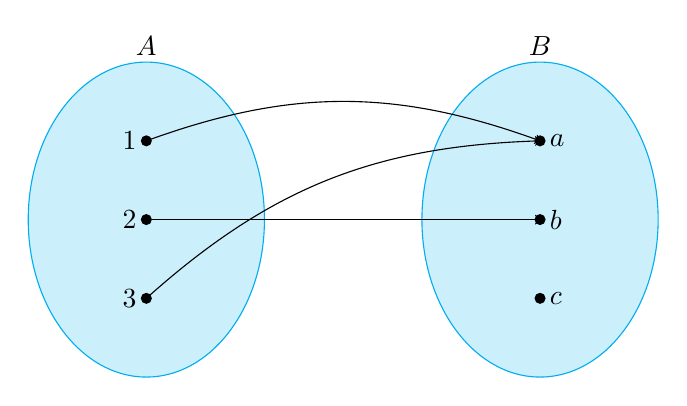
\begin{tikzpicture}
    % Aの集合
    \draw[fill=cyan!20, draw=cyan] (-2,0) ellipse (1.5cm and 2cm);
    \node at (-2,2.2) {$A$};

    % Bの集合
    \draw[fill=cyan!20, draw=cyan] (3,0) ellipse (1.5cm and 2cm);
    \node at (3,2.2) {$B$};

    % Aの要素
    \fill (-2,1) circle (2pt);
    \node[left] at (-2,1) {$1$};

    \fill (-2,0) circle (2pt);
    \node[left] at (-2,0) {$2$};

    \fill (-2,-1) circle (2pt);
    \node[left] at (-2,-1) {$3$};

    % Bの要素
    \fill (3,1) circle (2pt);
    \node[right] at (3,1) {$a$};

    \fill (3,0) circle (2pt);
    \node[right] at (3,0) {$b$};

    \fill (3,-1) circle (2pt);
    \node[right] at (3,-1) {$c$};

    % 矢印(写像)
    \draw[->, thin] (-2,1) to[bend left=20] (3,1); % 1をaに対応
    \draw[->, thin] (-2,0) to[bend left=0] (3,0); % 2をbに対応
    \draw[->, thin] (-2,-1) to[bend left=20] (3,1); % 3をaに対応
  \end{tikzpicture}
  \caption{写像 $f \colon A \to B$}
\end{figure}

この例では,$1$と$3$がともに$a$に対応しているが,上記の写像の定義ではこのような場合があってもよい.
また,$A$のどの元にも対応しない元$c$の存在も許容される.

学習が進むと,「任意の$ a_1 , a_2 \in A$に対して,$ a_1 \ne a_2$ならば$f(a_1) \ne f(a_2)$である写像」や
「任意の$ b \in B$に対して,ある$a \in A$が存在して,$b=f(a)$となる写像」を考える場合もあるが,この説明はもう少しあとにしよう.

\phantomsection
\subsubsection{写像の例}

ここでは直感的な理解を深めるために,具体例を挙げてみよう.

\begin{example}{自動販売機}{自動販売機}
  自動販売機には複数のボタンがあり,それぞれが特定の飲み物に対応している\footnote{ボタンをひとつ押しただけで何種類も飲み物が出てくる自動販売機はまずないであろう.少なくとも筆者は知らない.}.

  集合$A$を自動販売機のボタンの集合,集合$B$を提供される飲み物の集合としよう.各ボタン $a \in A$ に対して,そのボタンを押すと出てくる飲み物を $b \in B$ とする.

  このとき,
  \[
    b=f(a)
  \]
  とかくと,$f$ は写像の定義を満たす.
\end{example}


\subsubsection{像(値域)と逆像}

\begin{definition}{像(値域)}{像(値域)}
  写像$f \colon A \to B$において,集合$A$の部分集合$A' \subset A$に対する\emph{像}(\emph{値域})$f(A')$とは,
  \[
    f(A') = \{ f(a) \mid a \in A' \}
  \]
  で定義される集合である.特に,$A' = A$のときの$f(A)$を$f$の\emph{像}(\emph{値域})という.

  \index{ぞう@像} \index{ちいき@値域}
\end{definition}

\begin{figure}[h]
  \centering
  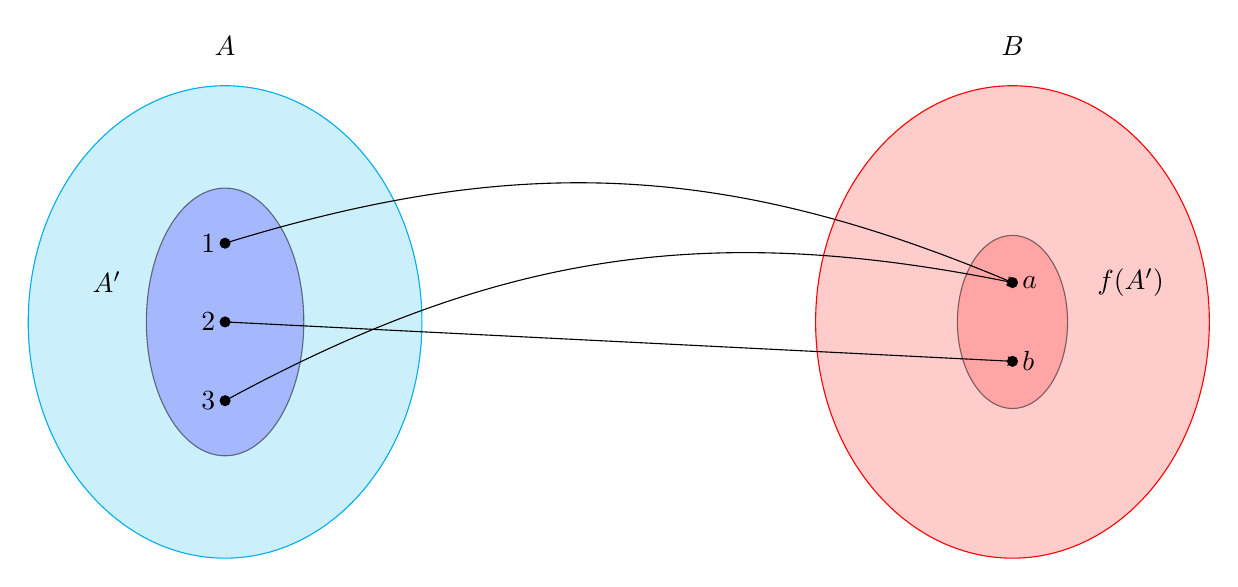
\begin{tikzpicture}[scale=1]
    % Aの集合(薄い青色)
    \draw[fill=cyan!20, draw=cyan] (-5,0) ellipse (2.5cm and 3cm);
    \node at (-5,3.5) {$A$};

    % Bの集合(薄い赤色)
    \draw[fill=red!20, draw=red] (5,0) ellipse (2.5cm and 3cm);
    \node at (5,3.5) {$B$};


        % A'の集合(濃い青色)
    \draw[fill=blue!50, opacity=0.5] (-5,0) ellipse (1.0cm and 1.7cm);
    \node at (-6.5,0.5) {$A'$};

    % 像 f(A')(濃い赤色)
    \draw[fill=red!50, opacity=0.5] (5,0) ellipse (0.7cm and 1.1cm);
    \node at (6.5,0.5) {$f(A')$};


    % Aの要素
    \fill (-5,1) circle (2pt);
    \node[left] at (-5,1) {$1$};

    \fill (-5,0) circle (2pt);
    \node[left] at (-5,0) {$2$};

    \fill (-5,-1) circle (2pt);
    \node[left] at (-5,-1) {$3$};

    % Bの要素
    \fill (5,0.5) circle (2pt);
    \node[right] at (5,0.5) {$a$};

    \fill (5,-0.5) circle (2pt);
    \node[right] at (5,-0.5) {$b$};


    % 矢印(写像)
    \draw[->, thin] (-5,1) to[bend left=20] (5,0.5); % 1をaに対応
    \draw[->, thin] (-5,0) to[bend left=0] (5,-0.5); % 2をbに対応
    \draw[->, thin] (-5,-1) to[bend left=20] (5,0.5); % 3をaに対応
  \end{tikzpicture}
  \caption{像}
\end{figure}


\begin{definition}{逆像}{逆像}
  写像$f \colon A \to B$と集合$B' \subset B$に対して,$B'$の\emph{逆像}とは,
  \[
    f^{-1}(B') = \{ a \in A \mid f(a) \in B' \}
  \]
  で定義される集合である.

  \index{ぎゃくぞう@逆像}
\end{definition}

\begin{mycolumn}
  \deref{逆像}て定義した逆像は「写像」ではなく,あくまで「集合」であることに注意したい.
  逆像と紛らわしい単語に「逆写像」があるが,逆写像は$f$が全単射であるときに定義される写像である.その一方で,逆像は$f$が全単射でなくても定義される.
\end{mycolumn}


\begin{figure}[h]
  \centering
  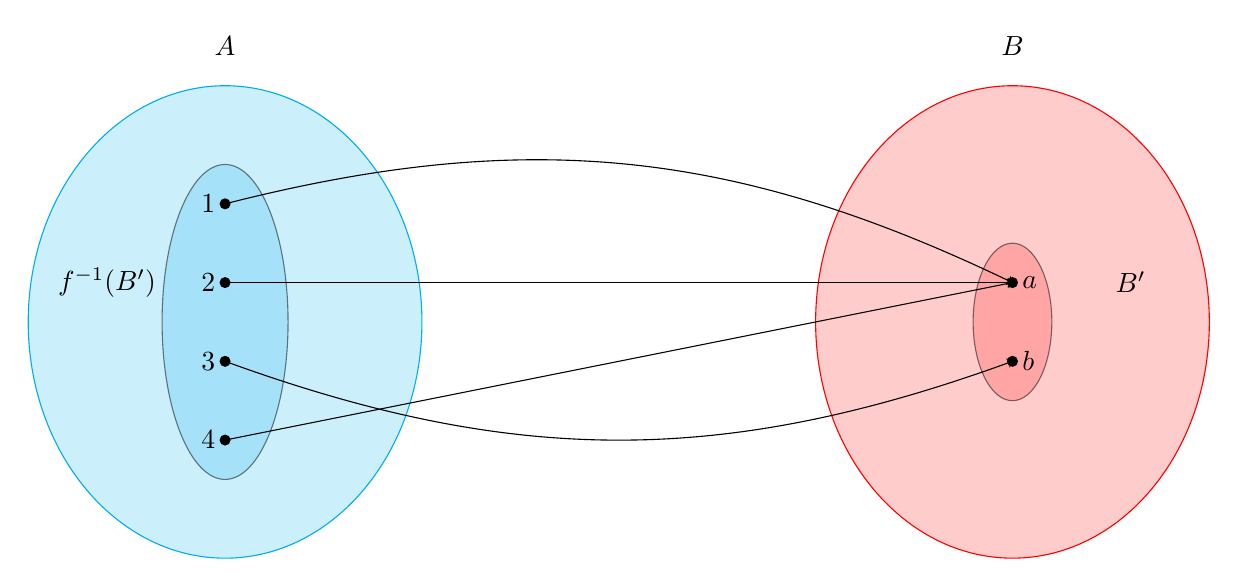
\begin{tikzpicture}[scale=1]
    % 集合 A の描画(薄い青色)
    \draw[fill=cyan!20, draw=cyan] (-5,0) ellipse (2.5cm and 3cm);
    \node at (-5,3.5) {$A$};

    % 集合 B の描画(薄い赤色)
    \draw[fill=red!20, draw=red] (5,0) ellipse (2.5cm and 3cm);
    \node at (5,3.5) {$B$};

    % B' の集合(濃い赤色)
    \draw[fill=red!50, opacity=0.5] (5,0) ellipse (0.5cm and 1.0cm);
    \node at (6.5,0.5) {$B'$};

    % f^{-1}(B') の集合(濃い青色)
    \draw[fill=cyan!50, opacity=0.5] (-5,0) ellipse (0.8cm and 2cm);
    \node at (-6.5,0.5) {$f^{-1}(B')$};

    % A の要素
    \fill (-5,1.5) circle (2pt);
    \node[left] at (-5,1.5) {$1$};

    \fill (-5,0.5) circle (2pt);
    \node[left] at (-5,0.5) {$2$};

    \fill (-5,-0.5) circle (2pt);
    \node[left] at (-5,-0.5) {$3$};

    \fill (-5,-1.5) circle (2pt);
    \node[left] at (-5,-1.5) {$4$};

    % B の要素
    \fill (5,0.5) circle (2pt);
    \node[right] at (5,0.5) {$a$};

    \fill (5,-0.5) circle (2pt);
    \node[right] at (5,-0.5) {$b$};

    % 矢印(写像 f)
    \draw[->, thin] (-5,1.5) to[bend left=20] (5,0.5); % 1 を a に対応
    \draw[->, thin] (-5,0.5) to[bend left=0] (5,0.5);   % 2 を a に対応
    \draw[->, thin] (-5,-0.5) to[bend right=20] (5,-0.5);% 3 を b に対応
    \draw[->, thin] (-5,-1.5) to[bend left=0] (5,0.5);% 4 を a に対応
  \end{tikzpicture}
  \caption{逆像}
\end{figure}



\subsubsection{単射\index{たんしゃ@単射}}

\begin{definition}{単射}{単射}
  写像$f$が$A$から$B$への単射であるとは,異なる要素$a_1, a_2 \in A$に対して,$f(a_1) \ne f(a_2)$が成り立つことである\footnote{この条件は,先の定義の対偶を考えると「$f(a_1) =f(a_2)$ならば$a_1=a_2$が成り立つ」とも言い換えられる.}.
\end{definition}

集合 $A = \{1, 2, 3\}$,$B = \{a, b, c, d\}$ を考え,写像 $f$ を以下のように定義する.
\[
  f(1) = a, \quad f(2) = b, \quad f(3) = c.
\]

\begin{figure}[h]
  \centering
  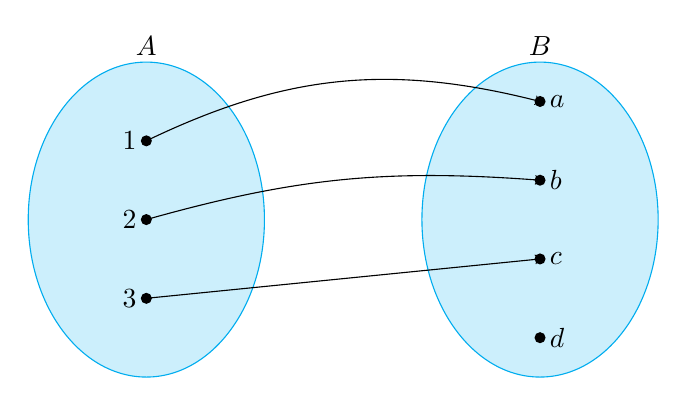
\begin{tikzpicture}
    % Aの集合
    \draw[fill=cyan!20, draw=cyan] (-2,0) ellipse (1.5cm and 2cm);
    \node at (-2,2.2) {$A$};

    % Bの集合
    \draw[fill=cyan!20, draw=cyan] (3,0) ellipse (1.5cm and 2cm);
    \node at (3,2.2) {$B$};

    % Aの要素
    \fill (-2,1) circle (2pt);
    \node[left] at (-2,1) {$1$};

    \fill (-2,0) circle (2pt);
    \node[left] at (-2,0) {$2$};

    \fill (-2,-1) circle (2pt);
    \node[left] at (-2,-1) {$3$};

    % Bの要素
    \fill (3,1.5) circle (2pt);
    \node[right] at (3,1.5) {$a$};

    \fill (3,0.5) circle (2pt);
    \node[right] at (3,0.5) {$b$};

    \fill (3,-0.5) circle (2pt);
    \node[right] at (3,-0.5) {$c$};

    \fill (3,-1.5) circle (2pt);
    \node[right] at (3,-1.5) {$d$};

    % 矢印(写像)
    \draw[->, thin] (-2,1) to[bend left=20] (3,1.5); % 1をaに対応
    \draw[->, thin] (-2,0) to[bend left=10] (3,0.5); % 2をbに対応
    \draw[->, thin] (-2,-1) to[bend right=0] (3,-0.5); % 3をcに対応
  \end{tikzpicture}
  \caption{単射の例}
\end{figure}

この$f$は単射だが,全射でない.

\begin{example}{電話番号と電話機}{電話番号と電話機}
  現代では,各電話番号は特定の電話機に対応している.この対応関係を写像として考えてみよう.

  集合$A$を電話番号の集合,集合$B$を実際の電話機の集合とする.
  また,電話番号 $a \in A$ に対して,$f$という規則で対応する電話機を $b \in B$ とする.

  このとき,
  \[
    b = f(a)
  \]
  とかくと,$f$ は写像の定義を満たす.

  また,現代では各電話番号が唯一の電話機に割り当てられることが多いため,異なる電話番号が同じ電話機を指し示すことはない.

  例えば,$A = \{\text{090-1234-5678}, \text{080-9876-5432}, \text{070-1111-2222}\}$,
  $B = \{\text{Phone1}, \text{Phone2}, \text{Phone3}\}$ とし,写像 $f$ を次のように定義する.
  \[
    f(\text{090-1234-5678}) = \text{Phone1}, \quad
    f(\text{080-9876-5432}) = \text{Phone2}, \quad
    f(\text{070-1111-2222}) = \text{Phone3}.
  \]

  このとき,$f$は単射である.
\end{example}

\subsubsection{全射\index{ぜんしゃ@全射}}

\begin{definition}{全射}{全射}
  写像$f$が$A$から$B$への全射であるとは,任意の$b \in B$に対して,ある$a \in A$が存在して,$f(a) = b$が成り立つことである.
\end{definition}

集合 $A = \{1, 2, 3\}$,$B = \{a, b\}$ を考え,写像 $f$ を以下のように定義する.
\[
  f(1) = a, \quad f(2) = a, \quad f(3) = b.
\]

\begin{figure}[h]
  \centering
  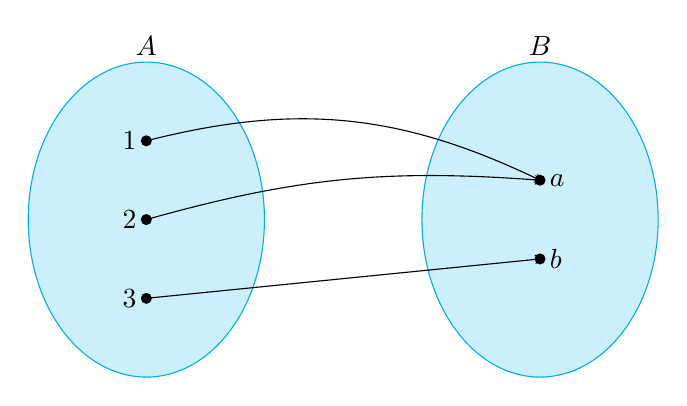
\begin{tikzpicture}
    % Aの集合
    \draw[fill=cyan!20, draw=cyan] (-2,0) ellipse (1.5cm and 2cm);
    \node at (-2,2.2) {$A$};

    % Bの集合
    \draw[fill=cyan!20, draw=cyan] (3,0) ellipse (1.5cm and 2cm);
    \node at (3,2.2) {$B$};

    % Aの要素
    \fill (-2,1) circle (2pt);
    \node[left] at (-2,1) {$1$};

    \fill (-2,0) circle (2pt);
    \node[left] at (-2,0) {$2$};

    \fill (-2,-1) circle (2pt);
    \node[left] at (-2,-1) {$3$};

    % Bの要素
    \fill (3,0.5) circle (2pt);
    \node[right] at (3,0.5) {$a$};

    \fill (3,-0.5) circle (2pt);
    \node[right] at (3,-0.5) {$b$};

    % 矢印(写像)
    \draw[->, thin] (-2,1) to[bend left=20] (3,0.5); % 1をaに対応
    \draw[->, thin] (-2,0) to[bend left=10] (3,0.5); % 2をaに対応
    \draw[->, thin] (-2,-1) to[bend right=0] (3,-0.5); % 3をbに対応
  \end{tikzpicture}
  \caption{全射の例}
\end{figure}

この$f$は全射だが,単射でない.

\begin{example}{分類コードと本}{分類コードと本}
  公共図書館では,各本に分類コードが割り当てられており,本を分類している.この対応関係を写像として考えてみよう.

  集合$A$を図書館にある本の集合,集合$B$を使用されている分類コードの集合とする.
  また,本 $a \in A$ に対して,分類コード $b \in B$ を割り当てる規則$f$を定める.

  このとき,
  \[
    b = f(a)
  \]
  と書くと,$f$ は写像の定義を満たす.

  図書館では,複数の本が同じ分類コードを持つことが一般的である、つまり,異なる本が同じ分類コードに対応することがある.

  例えば,$A = \{\text{『数学入門』}, \text{『微分積分』}, \text{『物理学基礎』}, \text{『統計学』}\}$,
  $B = \{\text{410}, \text{420}, \text{350}\}$ とし,写像 $f$ を次のように定義する.
  \[
    f(\text{『数学入門』}) = 410, \quad
    f(\text{『微分積分』}) = 410, \quad
    f(\text{『物理学基礎』}) = 420, \quad
    f(\text{『統計学』}) = 350.
  \]

  このとき,$f$は全射である.なぜなら,$B$の要素である410, 420, 350は全て$A$の要素によってカバーされているからである.しかし,$f$は単射ではない.なぜなら,$\text{『数学入門』}$と$\text{『微分積分』}$がともに410に対応しており,異なる本が同じ分類コードに対応しているからである.

\end{example}


\subsubsection{全単射\index{ぜんたんしゃ@全単射}}

\begin{definition}{全単射}{全単射}
  写像$f$が$A$から$B$への全単射であるとは,$f$が単射かつ全射となることである.
\end{definition}

集合 $A = \{1, 2, 3\}$,$B = \{a, b, c\}$ を考え,写像 $f$ を以下のように定義する.
\[
  f(1) = c, \quad f(2) = b, \quad f(3) = a.
\]

\begin{figure}[ht]
  \centering
  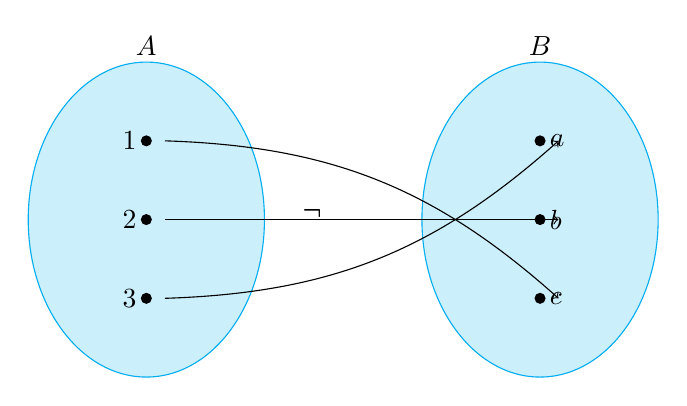
\begin{tikzpicture}
    % Aの集合
    \draw[fill=cyan!20, draw=cyan] (-2,0) ellipse (1.5cm and 2cm);
    \node at (-2,2.2) {$A$};

    % Bの集合
    \draw[fill=cyan!20, draw=cyan] (3,0) ellipse (1.5cm and 2cm);
    \node at (3,2.2) {$B$};

    % Aの要素
    \fill (-2,1) circle (2pt);
    \node[left] at (-2,1) {$1$};

    \fill (-2,0) circle (2pt);
    \node[left] at (-2,0) {$2$};

    \fill (-2,-1) circle (2pt);
    \node[left] at (-2,-1) {$3$};

    % Bの要素
    \fill (3,1) circle (2pt);
    \node[right] at (3,1) {$a$};

    \fill (3,0) circle (2pt);
    \node[right] at (3,0) {$b$};

    \fill (3,-1) circle (2pt);
    \node[right] at (3,-1) {$c$};
    ¬
    % 矢印(写像)
    \draw[->, thin] (-2,1) to[bend left=20] (3,-1); % 1をaに対応
    \draw[->, thin] (-2,0) to[bend left=0] (3,0); % 2をbに対応
    \draw[->, thin] (-2,-1) to[bend right=20] (3,1); % 3をcに対応
  \end{tikzpicture}
  \caption{全単射の例}
\end{figure}

この $f$ は単射かつ全射,すなわち全単射である.

\begin{example}{学籍番号と学生}{学籍番号と学生}
  あるクラスの学生とその学籍番号の対応を考える.
  集合 $A$ を学生の集合,集合 $B$ を学籍番号の集合とする.
  ここでは,
  \[
    A = \{\text{Alice}, \text{Bob}, \text{Charlie}\}, \quad
    B = \{\text{2024001}, \text{2024002}, \text{2024003}\}.
  \]
  とする.

  そして,学生 $a \in A$ に対して学籍番号 $b \in B$ を一意的に割り当てる規則 $f$ を次のように定義する.
  \[
    f(\text{Alice}) = \text{2024001}, \quad
    f(\text{Bob}) = \text{2024002}, \quad
    f(\text{Charlie}) = \text{2024003}.
  \]

  この写像 $f$ は$f$ は単射かつ全射,すなわち全単射である.
\end{example}

\begin{example}{単射・全射・全単射}{単射・全射・全単射}
  \begin{enumerate}[(A)]
    \item
          \[
            f \colon [0,\infty) \ni x \mapsto x^2  \in \mathbb{R}
          \]
          は単射であるが全射でない.
    \item
          \[
            g \colon \mathbb{R} \ni x \mapsto x^3 -3x^2 -9 \in \mathbb{R}
          \]
          は全射であるが単射でない.
    \item
          \[
            h  \colon \mathbb{R} \ni x \mapsto  2 \sin x \in  \mathbb{R}
          \]
          は全射でも単射でもない.しかし,
          \[
            h'  \colon [-\pi/2 , \pi/2 ]  \ni x \mapsto  2 \sin  x  \in [-2,2]
          \]
          は全単射である.
  \end{enumerate}
  \end{example}